\documentclass[a4paper,12pt]{article}
\setlength{\oddsidemargin}{-0.33in}
\setlength{\evensidemargin}{0in}
\setlength{\textwidth}{7in}
\setlength{\textheight}{10.2in}
\setlength{\footskip}{.5in}

\setlength{\voffset}{-.5in}
\setlength{\topmargin}{-0.5in}
\setlength{\headheight}{.5in}
\setlength{\headsep}{12pt}

\setlength\parindent{0pt}

% \usepackage{savetrees}
\usepackage{tikz}
\usepackage{stmaryrd}
\usepackage{hyperref}
\usepackage{color}
\usepackage{outlines}
\usepackage{rotating}
\usepackage{overpic}
\usepackage{algorithm}
\usepackage{algorithmic}
\usepackage{amsmath}
\usepackage{amssymb}
\usepackage{fancyhdr,lastpage}
\usepackage{enumerate}
\usepackage{graphicx}
\usepackage{epstopdf}
\usepackage{rotating}
\usepackage{mathrsfs}
\usepackage{tipa}
\usepackage{setspace}
\usepackage{natbib}
\usepackage{cancel}
\usepackage{mathtools}


%\doublespacing
\newcommand{\bs}[1]{\boldsymbol{#1}}
\newcommand{\real}[1]{\Re\left\{#1\right\}}
\newcommand{\TD}[2]{\frac{D#1}{D#2}}
\newcommand{\td}[2]{\frac{d#1}{d #2}}
\newcommand{\pd}[2]{\frac{\partial #1}{\partial #2}}
\newcommand{\pdd}[3]{\frac{\partial^2 #1}{\partial #2 \partial #3}}
\newcommand{\pdt}[2]{\frac{\partial^2 #1}{\partial #2 ^2}}
\newcommand{\expv}[1]{\left \langle #1 \right \rangle}
\newcommand{\tensort}[1]{\underline{\underline{#1}}}
\newcommand{\erf}[1]{\mbox{erf}{\left( {#1}\right)}}
\newcommand{\erfc}[1]{\mbox{erfc}{\left( {#1}\right)}}
\newcommand{\ands}{ \ \ \ \mbox{ and } \ \ \ }
\newcommand{\spword}[1]{ \ \ \ \mbox{ {#1} } \ \ \ }

\begin{document}
\title{Automatic Differentiation for Inverse Modeling Notes}
\author{Toby Harvey}
\maketitle
\vspace{-1cm}

\section{Introduction}

Some parameters in ice sheet models are hard if not impossible to observe. One strategy for estimating these parameters is to systematically adjust them so that outputs of the model best fit data that is observable. A cost function $\mathcal{J}(\alpha, u^{obs}, \hat{u}(\alpha))$, where $\alpha$ is the model parameter, is used to quantify the error between the model outputs $\hat{u}$ and the observable data $u^{obs}$. Most methods of minimizing $\mathcal{J}$ (gradient decent, etc...) require taking the derivative of the cost function with respect to the parameter, $\frac{d\mathcal{J}}{d\alpha}$. By the chain rule this is computed as:

\begin{align*}
  \frac{d\mathcal{J}}{d\alpha} = \pd{\mathcal{J}}{\alpha} + \pd{\mathcal{J}}{\hat{u}}\pd{\hat{u}}{\alpha}.
\end{align*}

The first two derivatives are easy to compute analytically, but the 3rd one is much harder. One possible solution is to try to compute it via perturbing the parameter of interest slightly and taking a finite difference:

\begin{align*}
  \pd{\hat{u}}{\alpha} \approx \frac{\hat{u}^{pert} - \hat{u}}{\alpha^{pert} - \alpha}.
\end{align*}

This requires running your model at least twice to compute a gradient for a single parameter, and in the case of a spatially variable parameter at least $n$ times where $n$ is the number of spatial degrees of freedom. The adjoint method is a method that requires more mathematical machineary, but requires solving only one additional model/system. The problem here is that it can be very difficult, if not impossible to derive this system. A third technique, automatic differentiation (AD), is summerized here. It is automatic in the sense that nothing coming from the specfic model system has to be derived, although it is more expensive than the adjoint method. First I describe automatic differentiation usinng a toy example, then explain how it is applied to a full forward model code.


\section{Automatic Differentiation of a Simple Code/Function}


Lets say we write a code that computes a very simple function:

\begin{align*}
  y = f(x_1, x_2, x_3) = x_1x_2 + \sin(x_3) - \log(x_1).
\end{align*}

at its essence, regardless of language or computer architecture, we need to follow the dependency graph in figure \ref{fig:comp-graph}. If we take this as our primary (think forward model) code, we can have a secondary code that, at runtime builds, the dependancy graph in the background. This is the AD code.

\begin{figure}
\centering
\begin{tikzpicture}[
  roundnode/.style={circle, draw=black, very thick, minimum size=7mm},
  squarednode/.style={rectangle, draw=black, very thick, minimum size=7mm},
]

\node[roundnode] (x1) at (0,0) {$x_1$};
\node[roundnode] (x2) at (3,0) {$x_2$};
\node[roundnode] (x3) at (6,0) {$x_3$};

\node[squarednode] (mul) at (3,-2) {$v_2 = x_1 x_2$};
\node[squarednode] (sin) at (6,-2) {$v_3 = \sin(x_3)$};
\node[squarednode] (log) at (0,-2) {$v_1 = \log(x_1)$};

\node[squarednode] (sum1) at (3.75,-3.5) {$v_4 = v_2+ v_3$};

\node[squarednode] (y) at (3.75,-5) {$y = v_4 - v_1$};

\draw[->] (x1) -- (mul);
\draw[->] (x2) -- (mul);
\draw[->] (x3) -- (sin);

\draw[->] (mul) -- (sum1);
\draw[->] (sin) -- (sum1);

\draw[->] (x1) -- (log);
\draw[->] (sum1) -- (y);
\draw[->] (log) -- (y);

\end{tikzpicture}
\caption{computational dependency graph of $y = x_1 x_2 + \sin(x_3) - \log(x_1)$.}
\label{fig:comp-graph}
\end{figure}

\section{Automatic Differentiation of a Forward Model}


\end{document}


